\documentclass[11pt]{amsbook}

\usepackage{../HBSuerDemir}	% ------------------------

\begin{document}

% ++++++++++++++++++++++++++++++++++++++
\hPage{feyzioglu/88}
% ++++++++++++++++++++++++++++++++++++++

and the arrangement $k_1 , \dots k_{j-1} , k_{j+1} , \dots , k_n$ of the numbers $1 , 2 , \dots , n-1$ we
have $a_{k_i} \dots a_{k_{j-1}} a_{k_{j+1}} \dots a_{k_n} = a_1 a_2 \dots a_{n-1}$; therefore
\begin{align*}
	a_{k_1} a_{k_2} \dots a_{k_n} &= (a_{k_i} \dots a_{k_{j-1}} a_{k_{j+1}} \dots a_{k_n}) a_n \\
	&= (a_1 a_2 \dots a_{n-1}) a_n \\
	&= a_1 a_2 \dots a_{n-1} a_n
\end{align*}
and the induction argument goes through. In the chain equations
above, the term $(a_{k_1} \dots a_{k_{j-1}})$ is absent if $j = 1$ and the term $(a_{k_{j+1}} \dots a_{k_n})$ is
absent if $j = n$. The argument remains valid in these cases. \footnote{This proof continues from the previous page.}
\\
\textbf{8.13 Lemma:} Let G be a commutative group and let $a_1 , a_2, \dots , a_n$ be arbitrary
elements of G. Then
\[
	a_{k_1} a_{k_2} \dots a_{k_n} = a_1 a_2 \dots a_{n-1} a_n
\]
for all arrangements $k_1,k_2, \dots ,k_n$ of the indices $1,2, \dots n$.
\begin{proof}
	This follows immediately from Lemma 8.12.
\end{proof}
\textbf{8.14 Lemma:} Let $G$ be a nonempty set with an associative multiplication
on it and let $a,b \in G$.
\\
(1) If $ab = ba$, then $(ab)^n = a^n b^n$ for all $n \in N$.
\\
(2) If, in addition, there is a unique $e \in G$ such that $ce = ec$ for all $c \in G$,
and if we put $c^0 = e$ for all $c \in G$, then $(ab)^0 = a^0 b^0$.
\\
(3) If, in addition, G is a group, then $(ab)^n = a^n b^n$ for all $n \in Z$.
\begin{proof}
	(1) The claim is trivially true when $n = 1$. Suppose now $n \geq 2$ and
	assume $(ab)^{n-1} = a^{n-1} b^{n-1}$. Then
	\begin{align*}
		(ab)^n = (ab)^{n-1} (ab) &= (a^{n-1} b^{n-1}) (ab) \\
		&= a^{n-1}(b^{n-1} a) b \\
		&= a^{n-1} (a b^{n-1})b && \text{(by Lemma 8.10)} \\
		&= (a^{n-1}a)(b^{n-1}b) \\
		&= a^n b^n
	\end{align*}
	and the claim is true for $n$. So $(ab)^n = a^n b^n$ for all $n \in N$.
	\\
	(2) Writing $e$ for $c$, we get $ee = e$. Thus $(ab)^0 = e = ee = a^0 e = a^0 b^0$.
	\\
	(3) That $(ab)^n = a^n b^n$ is proved for $n \geq 0$. We are to prove it also when $n \leq -1$. Replacing $n$ by $-n$, we are to prove that $(ab)^{-n} = a^{-n} b^{-n}$ for $n \in N$. We note that $ab = ba$ implies $b^{-1} a^{-1} = (ab)^{-1} = (ba)^{-1} = a^{-1} b^{-1}$, so the
\end{proof}

% =======================================================
\end{document}  

%==== templates ====

%==== environments ====

%\begin{figure}[htb]
%	\centering
%	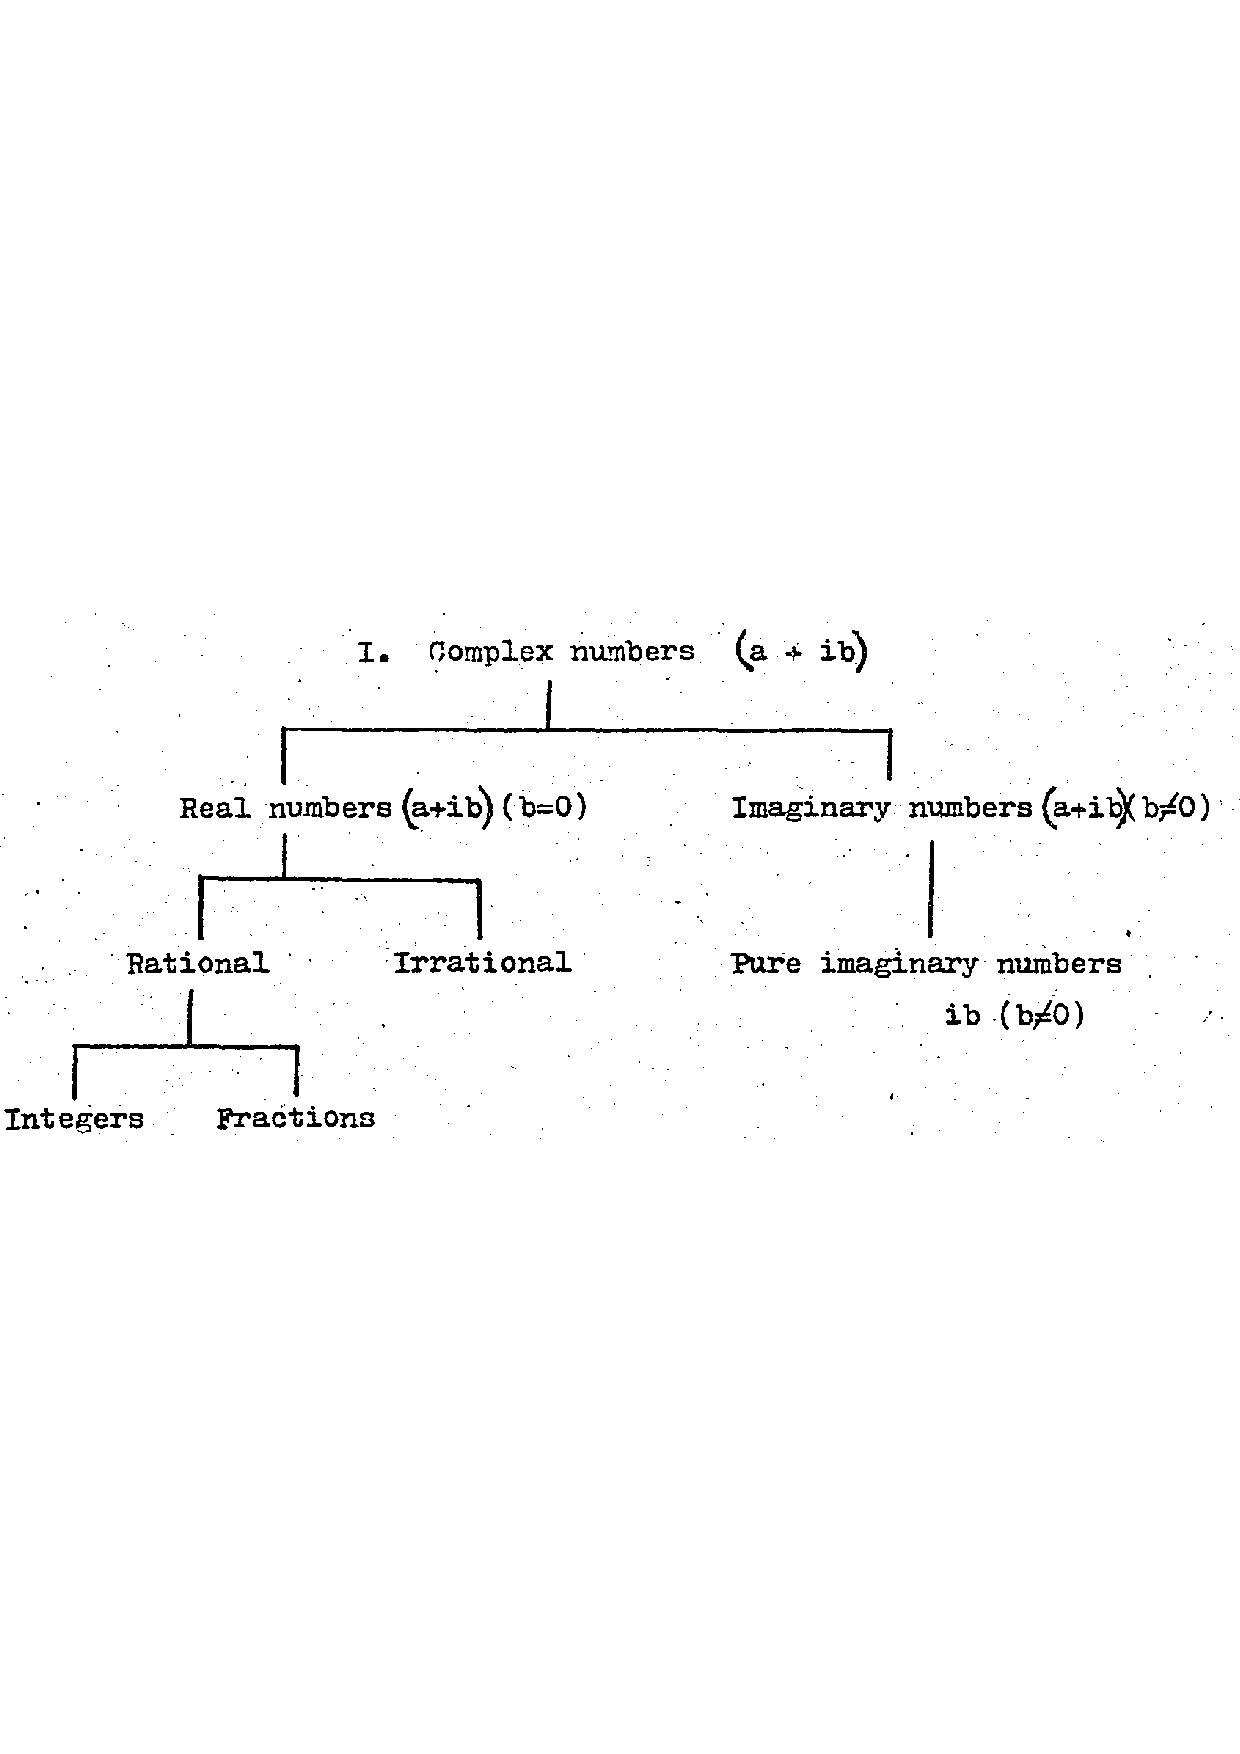
\includegraphics[width=0.9\textwidth]{images/SD-1-1p15A}
%	\caption{Classification of complex numbers}
%	\label{fig:classificationOfComplexNumbersA}
%\end{figure}

%\begin{center}
%\begin{tabular}{cc}
%\end{tabular}
%\end{center}

%\begin{exmp}
%\begin{hSolution}
%\end{hSolution}
%\end{exmp}

%\begin{hEnumerateAlpha}
%\end{hEnumerateAlpha}

%\begin{hEnumerateRoman}
%\end{hEnumerateRoman}

%$
%\begin{bmatrix}
%\end{bmatrix}
%$

%\frac{aaaa}{bbb}
%\frac{a_{n}}{b_{n}}
%\left( aaaa \right)
%\Longrightarrow

%\begin{multicols}{2}
%	bb
%\columnbreak
%	aa
%\end{multicols}
